\documentclass[]{book}
\usepackage{lmodern}
\usepackage{amssymb,amsmath}
\usepackage{ifxetex,ifluatex}
\usepackage{fixltx2e} % provides \textsubscript
\ifnum 0\ifxetex 1\fi\ifluatex 1\fi=0 % if pdftex
  \usepackage[T1]{fontenc}
  \usepackage[utf8]{inputenc}
\else % if luatex or xelatex
  \ifxetex
    \usepackage{mathspec}
  \else
    \usepackage{fontspec}
  \fi
  \defaultfontfeatures{Ligatures=TeX,Scale=MatchLowercase}
\fi
% use upquote if available, for straight quotes in verbatim environments
\IfFileExists{upquote.sty}{\usepackage{upquote}}{}
% use microtype if available
\IfFileExists{microtype.sty}{%
\usepackage[]{microtype}
\UseMicrotypeSet[protrusion]{basicmath} % disable protrusion for tt fonts
}{}
\PassOptionsToPackage{hyphens}{url} % url is loaded by hyperref
\usepackage[unicode=true]{hyperref}
\hypersetup{
            pdftitle={Genomics Boot Camp},
            pdfauthor={Gábor Mészáros},
            pdfborder={0 0 0},
            breaklinks=true}
\urlstyle{same}  % don't use monospace font for urls
\usepackage{natbib}
\bibliographystyle{apalike}
\usepackage{color}
\usepackage{fancyvrb}
\newcommand{\VerbBar}{|}
\newcommand{\VERB}{\Verb[commandchars=\\\{\}]}
\DefineVerbatimEnvironment{Highlighting}{Verbatim}{commandchars=\\\{\}}
% Add ',fontsize=\small' for more characters per line
\usepackage{framed}
\definecolor{shadecolor}{RGB}{248,248,248}
\newenvironment{Shaded}{\begin{snugshade}}{\end{snugshade}}
\newcommand{\KeywordTok}[1]{\textcolor[rgb]{0.13,0.29,0.53}{\textbf{#1}}}
\newcommand{\DataTypeTok}[1]{\textcolor[rgb]{0.13,0.29,0.53}{#1}}
\newcommand{\DecValTok}[1]{\textcolor[rgb]{0.00,0.00,0.81}{#1}}
\newcommand{\BaseNTok}[1]{\textcolor[rgb]{0.00,0.00,0.81}{#1}}
\newcommand{\FloatTok}[1]{\textcolor[rgb]{0.00,0.00,0.81}{#1}}
\newcommand{\ConstantTok}[1]{\textcolor[rgb]{0.00,0.00,0.00}{#1}}
\newcommand{\CharTok}[1]{\textcolor[rgb]{0.31,0.60,0.02}{#1}}
\newcommand{\SpecialCharTok}[1]{\textcolor[rgb]{0.00,0.00,0.00}{#1}}
\newcommand{\StringTok}[1]{\textcolor[rgb]{0.31,0.60,0.02}{#1}}
\newcommand{\VerbatimStringTok}[1]{\textcolor[rgb]{0.31,0.60,0.02}{#1}}
\newcommand{\SpecialStringTok}[1]{\textcolor[rgb]{0.31,0.60,0.02}{#1}}
\newcommand{\ImportTok}[1]{#1}
\newcommand{\CommentTok}[1]{\textcolor[rgb]{0.56,0.35,0.01}{\textit{#1}}}
\newcommand{\DocumentationTok}[1]{\textcolor[rgb]{0.56,0.35,0.01}{\textbf{\textit{#1}}}}
\newcommand{\AnnotationTok}[1]{\textcolor[rgb]{0.56,0.35,0.01}{\textbf{\textit{#1}}}}
\newcommand{\CommentVarTok}[1]{\textcolor[rgb]{0.56,0.35,0.01}{\textbf{\textit{#1}}}}
\newcommand{\OtherTok}[1]{\textcolor[rgb]{0.56,0.35,0.01}{#1}}
\newcommand{\FunctionTok}[1]{\textcolor[rgb]{0.00,0.00,0.00}{#1}}
\newcommand{\VariableTok}[1]{\textcolor[rgb]{0.00,0.00,0.00}{#1}}
\newcommand{\ControlFlowTok}[1]{\textcolor[rgb]{0.13,0.29,0.53}{\textbf{#1}}}
\newcommand{\OperatorTok}[1]{\textcolor[rgb]{0.81,0.36,0.00}{\textbf{#1}}}
\newcommand{\BuiltInTok}[1]{#1}
\newcommand{\ExtensionTok}[1]{#1}
\newcommand{\PreprocessorTok}[1]{\textcolor[rgb]{0.56,0.35,0.01}{\textit{#1}}}
\newcommand{\AttributeTok}[1]{\textcolor[rgb]{0.77,0.63,0.00}{#1}}
\newcommand{\RegionMarkerTok}[1]{#1}
\newcommand{\InformationTok}[1]{\textcolor[rgb]{0.56,0.35,0.01}{\textbf{\textit{#1}}}}
\newcommand{\WarningTok}[1]{\textcolor[rgb]{0.56,0.35,0.01}{\textbf{\textit{#1}}}}
\newcommand{\AlertTok}[1]{\textcolor[rgb]{0.94,0.16,0.16}{#1}}
\newcommand{\ErrorTok}[1]{\textcolor[rgb]{0.64,0.00,0.00}{\textbf{#1}}}
\newcommand{\NormalTok}[1]{#1}
\usepackage{longtable,booktabs}
% Fix footnotes in tables (requires footnote package)
\IfFileExists{footnote.sty}{\usepackage{footnote}\makesavenoteenv{long table}}{}
\usepackage{graphicx,grffile}
\makeatletter
\def\maxwidth{\ifdim\Gin@nat@width>\linewidth\linewidth\else\Gin@nat@width\fi}
\def\maxheight{\ifdim\Gin@nat@height>\textheight\textheight\else\Gin@nat@height\fi}
\makeatother
% Scale images if necessary, so that they will not overflow the page
% margins by default, and it is still possible to overwrite the defaults
% using explicit options in \includegraphics[width, height, ...]{}
\setkeys{Gin}{width=\maxwidth,height=\maxheight,keepaspectratio}
\usepackage[normalem]{ulem}
% avoid problems with \sout in headers with hyperref:
\pdfstringdefDisableCommands{\renewcommand{\sout}{}}
\IfFileExists{parskip.sty}{%
\usepackage{parskip}
}{% else
\setlength{\parindent}{0pt}
\setlength{\parskip}{6pt plus 2pt minus 1pt}
}
\setlength{\emergencystretch}{3em}  % prevent overfull lines
\providecommand{\tightlist}{%
  \setlength{\itemsep}{0pt}\setlength{\parskip}{0pt}}
\setcounter{secnumdepth}{5}
% Redefines (sub)paragraphs to behave more like sections
\ifx\paragraph\undefined\else
\let\oldparagraph\paragraph
\renewcommand{\paragraph}[1]{\oldparagraph{#1}\mbox{}}
\fi
\ifx\subparagraph\undefined\else
\let\oldsubparagraph\subparagraph
\renewcommand{\subparagraph}[1]{\oldsubparagraph{#1}\mbox{}}
\fi

% set default figure placement to htbp
\makeatletter
\def\fps@figure{htbp}
\makeatother

\usepackage{booktabs}
\usepackage{amsthm}
\makeatletter
\def\thm@space@setup{%
  \thm@preskip=8pt plus 2pt minus 4pt
  \thm@postskip=\thm@preskip
}
\makeatother

\title{Genomics Boot Camp}
\author{Gábor Mészáros}
\date{2021-01-24}

\begin{document}
\maketitle

{
\setcounter{tocdepth}{1}
\tableofcontents
}
\chapter{Hello and welcome!}\label{hello-and-welcome}

If you are reading this, it means I managed to get everything into a
publishable resource. If it is good enough that is up to you to judge,
dear reader!

The contents and the writing style of the book are based on my teaching
experience of both theoretical background and practical data analysis
skills to a wide range of learners, starting from MSc level, to PhD
students and researchers of various overall experience in university and
stand-alone post-doc courses. The people I talked to were similar. They
were very interested to learn about the practical handling and analysis
of single nucleotide polymorphism (SNP) data, but for some reason, they
could not acquire enough practice, so far. Also, I noticed that
regardless of seniority level they appreciated simple and
straightforward examples, demonstrations, and in detail explanations of
seemingly simple issues (e.g.~why not to put space in a filename, what
is the file path, and others). Indeed, these topics need to be discussed
in detail to avoid unwelcome surprises later and enable to build a
steady knowledge of SNP data analysis practice.

This book and the affiliated
\href{https://www.youtube.com/channel/UCXuX-kQ1TbKHWeB75NgmhlA}{Genomics
Boot Camp YouTube channel} tries to follow this beginner friendly,
detailed discussion approach. Of course, there is plenty of topics that
could (and hopefully will) be discussed and shown, but for now, only a
subset is appearing in any of the resources. The goal was to put
together a resource on a need-to-know basis, presenting only the parts
that are necessary to achieve the goal. In particular, I wanted to avoid
the flood of information that might be interesting, might be even
useful, but at that point is not really necessary. With this said, I
plan to follow up with more topics that should cover all the basics, and
with time even more sophisticated approaches.

The Genomics Boot Camp is a resource that helps you to start your
journey in practical analysis of genomic data, with a focus on SNP data.
The chapters follow the same structure all the time: provide background
information and practical insight to the topic, and when appropriate
exercises to reinforce the obtained knowledge. The Genomics Boot Camp as
a whole was designed to cater to various learning preferences with
written text, video demonstrations, and the possibility of hands-on
exercises. There is a certain overlap between the book and the YouTube
channel contents, but each has unique pieces of information as well. So
for the full experience, I suggest checking out both.

The solutions for exercises are on the accompanying YouTube channel.
Apart from the exercise solutions, the contents of the YouTube channel
include more videos taking a deeper dive into more practical and
theoretical aspects of genomics. Beginner friendly, of course!

Due to the nature of genomics data and DNA being very similar in humans,
animals, microbes and, plants, the methods and approaches presented in
this book are usable for your favorite research organism. There is no
previous data analysis knowledge required to start. The plan is that you
acquire everything as you go along.

\section{Acknowledgements}\label{acknowledgements}

The visuals of is book are based on the bookdown-demo framework, by
Yihui Xie.

\section{Copyright}\label{copyright}

This book is licensed under the
\href{https://creativecommons.org/licenses/by-nc-nd/4.0/}{Creative
Commons Attribution-NonCommercial-NoDerivs 4.0 License (CC BY-NC-ND
4.0)}.

\chapter{Technical preparations}\label{technical-preparations}

\begin{quote}
\textbf{Learning outcomes} At the end of this chapter, you will be able
to recognize and avoid some of the most common mistakes in storing and
handling data. You will be able to name your files in a proper way and
to avoid potential future problems.
\end{quote}

\hypertarget{overall-recommendations-tips-and-tricks}{\section{Overall
recommendations, tips and
tricks}\label{overall-recommendations-tips-and-tricks}}

The motivation to write this section comes from my previous experiences
of the MSc level course I teach on Management and analysis of
high-density genomic data. During the lectures, I met students who in
the follow-up weeks became very versatile in simple analyses of genomic
data. So this was great! Most of them however had some pretty awful
habits when it came to their practices in data handling and storage. The
previous statement is less about criticism and more of a note that the
conventional user of a computer, especially on a Windows machine is just
spoiled. Everything works! We do not even need to think where our files
are, as we get there in a few clicks, or in the worst case we use the
built-in search functions.

You can, and \textbf{you have to do better} if you are even half serious
about genomic data analysis. This part will answer the questions of what
can you improve and what are the ``best'' ways to do that.

So let us consider a typical case: Student X is interested in genomic
data analysis and jumps right at the later chapters of this book. They
create a new folder on the Windows desktop called ``Genomic data
analysis'', where all data from all lectures gets copied, including
programs and scripts they write. This way they will know where things
are, should they ever need them again. There are multiple problems with
this approach. Let's see what these problems are and how could be
improved:

\textbf{Do not store anything on the desktop}

\begin{itemize}
\tightlist
\item
  Although it seems to be so close visually, the files on the Windows
  desktop are deeper in the computer's file structure. This might then
  introduce unnecessary complexity in your scripts when it comes to the
  definition of the file PATH
\item
  The easy point and click access also means that it is more easily
  deleted by an accident by you or others (the danger is especially high
  during home office sessions if there are small children around)
\end{itemize}

\textbf{Do not store anything of importance on the system drive (usually
C:)}

\begin{itemize}
\tightlist
\item
  In case of major problems this drive is the one that gets wiped first,
  so to avoid future hassle just avoid having anything there that you
  care about
\end{itemize}

\textbf{In case your computer has only a single drive - Use Backup}

\begin{itemize}
\tightlist
\item
  I can not stress enough how the backup of all important files. Even
  for the less important ones is absolutely crucial!
\item
  The C: drive can go down in a system failure, virus, or similar, but
  your work is not safe on other drives either
\item
  External hard drives and USB sticks are not a solution! These break
  down and get lost surprisingly easily, so arguably they are even worse
  than your laptop's drive
\item
  My strong suggestion is to use cloud storage services - even the free
  options give you enough space to keep your work safe
\end{itemize}

\textbf{Smart strategies to utilize cloud storage}

\begin{itemize}
\tightlist
\item
  Let's say you go on with the free version of your favorite service,
  which is typically not enough to store large amounts of data
\item
  You can use the cloud storage for your script files and other
  documents you write - these are typically very small files into which
  you invested a lot of your time. So they are on the top of your list
  when it comes to protection
\item
  You can even store crucial genotype data in a binary ped format (more
  on this later) which takes a very little HDD space
\end{itemize}

\textbf{One project - one folder}

\begin{itemize}
\tightlist
\item
  Unlike Student X, do not dump everything into one folder! It seems
  intuitive if you have one, maybe two things to analyze, but you
  quickly lose track afterward
\item
  As you will see in the future analyses, the programs tend to produce a
  lot of temporary files, or just files that you do not need. You might
  be even deleting some of them. In this process, it is way too easy to
  delete your script files, or pieces of the input data as well.
  \ldots{}and Pooof! there goes your whole day effort to put something
  meaningful together!
\item
  Of course, this does not apply if you set your recycle bin not to hard
  delete files right away, so ensure it is set this way.
\item
  Even if you do and kept my previous advice on cloud storage, you can
  use the ``undelete'' function of the Windows recycle bin to save the
  day
\item
  But even these Get-out-of-jail-free-cards do not solve our main
  problem of being lost and confused if you have 15 types of analyses in
  a folder, so just stick to the one folder per project
\end{itemize}

\textbf{Use folders within folders}

\begin{itemize}
\tightlist
\item
  Yes! You can even do more and better by a standard internal
  organization of your folder structures
\item
  There is a lot of room for experimentation and individual flavors
  here, but the two things I would suggest
\end{itemize}

** Folder for script files: These could be stored literally anywhere on
your computer and still work with any other data via a correctly set
PATH, so you might just store them in a secure (Backupped!) place. **
Folder for the original data: I like to keep separate original and
untouched data in its own folder. If anything happens during the
analyses (and trust me, a lot of very unexpected things tend to happen),
I can recreate everything with the original data and the saved script
files.

\textbf{Use descriptive and appropriate names for your files and
folders}

\begin{itemize}
\tightlist
\item
  This is a topic on its own with a lot of issues to unpack, so it is
  described in detail in the
  \protect\hyperlink{file-naming-conventions}{File naming conventions}
  part below.
\item
  To keep it short here, Student X in our example case just sets
  themself up for future problems using spaces in folder names, as this
  could backfire in unexpected ways. So don't use spaces in filenames.
\item
  Also, the name of the folder does not tell anything about its
  contents. You can spare yourself quite a bit of time in the future to
  take a bit of time now and give a very descriptive name with an
  obvious link to the content, e.g. ``2020\_pcaAustrianLeonbergerDogs''.
\end{itemize}

So these were my tips and tricks that you could consider when starting
out. They are based on my own experiences and the approaches I commonly
use. If you have other similar tips to share or discuss the ones
presented here, let me know via \href{https://twitter.com/GaborM_ABG}{my
Twitter}.

\hypertarget{file-naming-conventions}{\section{File naming
conventions}\label{file-naming-conventions}}

In this part of the Genomics Boot Camp, I want to elaborate on what the
PATH is, why is it useful for you to know about it, and what to keep in
mind when analyzing any kind of data. So first things first. The PATH
(written in all caps) is not the name of some sketchy religious
organization, but the set of directories where your executable files or
data are located. You can think of it as the address of the files on
your computer.

In most of the programs, you will work with you will have to specify
file locations on your computer. Therefore, it is good to know how does
it work and what conventions to follow, to avoid future problems.

There is a lot of freedom for self-expression and to include your own
spins and flavors when it comes to naming anything on your computer, but
there are a few basic rules you should abide by.

\textbf{Select a good location for your files}

As I suggested before in the
\protect\hyperlink{overall-recommendations-tips-and-tricks}{Overall
recommendations, tips and tricks}, it is a good thing to store your
files outside the system drive. In particular, the Desktop should be
avoided, as it includes your username, which can be tricky sometimes. It
might violate some of the rules established below.

\textbf{No spaces in file and folder names}

This by far the most common violation of good practices, when it comes
to beginner learners. Some programs became more forgiving in this
aspect, but avoiding spaces in names can spare you quite some headaches
on your data analysis journey.

\textbf{No special characters in filenames}

The most common case here is punctuation and brackets, but also special
characters of the various languages. My rule is to use only letters
available on the English keyboard.

\textbf{Use descriptive names}

Upon the first glance at the name of any file or folder, it should be
obvious to you (and any other person) what it contains. In this respect
names like ``final data'' or ``a.txt'' are pretty good examples, what
not to do. Try to give it a spin that falls into your flavor of naming
things, but also keeps the required amount of clarity.

\textbf{Naming conventions}

As for me, I like to use a combined system that sort of evolved as I
went along. For example, I have a folder for a project I work on called
``2015\_Appear\_LocaBreed''. There are several things to talk about
here.

When it comes to folder names, I picked up the habit of starting with a
number, which makes it easier to sort the folders and follow a certain
established logic. In the case of projects (as in the example), papers
or analyses I like to start with the year. This could be also a
sequential number, e.g.~a series of folders for paper submissions called
``1\_draft'', ``2\_submission'', ``3\_review''

You have surely noticed that none of these names contain any space, but
still are fairly easily readable. This is due to the naming conventions
used in these examples. And you can do it too!

Let's consider another example of a folder name:

sheepdiversityprojectlapampaargentina

The name is ok, but the readability is pretty horrible. We can improve
it a ton just by capitalizing the first letter in each word.

SheepDiversityProjectLaPampaArgentina

Much better, I believe! Still, we could add a few improvements. If you
have more similar folders at the same place, it might make sense to add
the relevant year. Also, one might argue that this particular name is
quite long, so we can break it a little bit by adding underscores.

2022\_SheepDiversityProject\_LaPampaArgentina

Even better! This is of course from my own perspective. You are free to
spin your own naming conventions around and experiment. There is also a
lot of guidelines on this available on the web that give helpful
suggestions. A nice and extensive
\href{https://www.huridocs.org/2016/07/file-naming-conventions-why-you-want-them-and-how-to-create-them/}{summary
can be found here}.

\hypertarget{basic-software}{\chapter{Basic
software}\label{basic-software}}

\begin{quote}
Learning outcomes At the end of this chapter you will be able to
recognize some of the software tools that do not come as pre-installed
with your operating system, but they are useful in handling and analysis
of genomic data.
\end{quote}

If you have not done any genomic data analysis on your computer before,
you probably have only the default set of programs installed. My guess
is MS Office or Open Office Suite for your general office needs, and the
Windows Notepad if you ever need to open a .txt file. You also probably
use Windows Explorer to move around the files or check search for them
if you are not certain where that pesky little document is located that
you need to email to somebody.

There is nothing wrong with this setup if you use your PC for office
work. If you want to work with genomic data, however, you can do better.

So before we jump into the specifics about genomic data, I want to talk
about my recommendations on which programs you should have on your
computer. These recommendations come from my own experience of working
with genomic data, as well as data handling and manipulation.

There are many possibilities for the software you can use, and these are
my personal favorites. I will talk about these below and briefly explain
why I like them.

I also want to add that these recommendations are written for an average
MS Windows user, as I assume most of you, dear learners, work in this
OS. Sadly, I am not aware of all the possibilities for Mac and Linux OS,
although versions or alternatives should exist.

\section{Text Editors}\label{text-editors}

The genotype files we will be dealing with are nothing else, but large
text files. Huge text files, sometimes. So it is inevitable to have text
editors to open them. Yes\ldots{} You want to use programming tools and
scripts to manipulate the files, but you also want to have the
possibility to open them and see if the contents are according to your
expectations. For this, you need a text editor. And no, the default
Windows Notepad is not a good tool to do this. A few brave souls even
try to use the WordPad, which is even worse.

As I mentioned before the genotype text files are often much larger than
you normally deal with. Instead of a few kilobytes, they often have a
few hundred megabytes or even a few gigabytes. In my experience, the
default tools struggle to open these.

You can do better\ldots{}

My first go-to \href{https://www.textpad.com/home}{program to open large
text files is TextPad}. This wonderful piece of software opens files in
size of gigabytes in a matter of seconds. It can also do a lot of other
things, such as file comparisons and some great text management moves,
which I do not fully utilize (meaning: I use it just to open and look at
the files).

The second \href{https://notepad-plus-plus.org/}{text editor I
frequently use is Notepad++}. I like it, in particular, to look at
various scripts, as the keywords in various programming languages are
highlighted via its color-coding system. Also, a lot of my time was
spared via its button ``Find {[}text{]} in All Opened Documents'', which
searches multiple files for expression and gives a clear overview of
findings. Can not recommend it enough\ldots{} Also, somehow I like the
visuals of this editor better.

\section{File management}\label{file-management}

We have to be very honest here\ldots{}

Most of the people who use the computer for ``ordinary'' school or
office work are not aware of the file structure and where are the files
stored on the computer. This is of course normally not a problem, but it
becomes an issue of sizeable proportions when you want to get even
half-serious about genomic data analysis. You can not even imagine how
many times I had to remind my students that the Desktop is not the place
to store your files and that they need to be aware of the file
structures and full file names they are working with. I honestly think
we are spoiled with the Windows (and probably also Mac) operating
systems, where everything just works even if we just click Next
\textgreater{} Next \textgreater{} Next and accept the default settings.

As an aspiring learner to analyze genomic data you can of course do
better\ldots{}

The first thing you can do is to \href{https://www.ghisler.com/}{install
Total Commander for your file management needs}. This is a great tool
that shows you the HDD and file structure of your computer, allows you
to copy and move files with ease. It also has a built-in file packing
and extraction tool, so you do not need to worry about having extra
software to install for that either. Another crucial thing is that it
allows you to see and edit file extensions! As you might or might not
know, in Windows each file comes with three, or sometimes four-letter
file extensions which are conveniently hidden in the default Windows
Explorer. This of course is not a problem for the common use of the
computer but could be (read: frequently is) a source of errors in data
analysis scripts for beginners. So again, I can not recommend this
enough\ldots{}

If you start to get low on hard disk space, a great program to utilize
is \href{https://windirstat.net/}{WinDirStat to visualize HDD use} via
color-coded boxes that are proportional to the size of the files. It
makes it very easy to see if you have any large files the removal of
which would help you in any way.

\textbf{Folder structure and backup}

Before you start any kind of analysis you need to think about the
structure you will be using.

One more recommendation for file management is to use cloud storage for
your crucial (or even all of your) files. Personally, I use Dropbox, but
of course, there are plenty of other services with the same
functionality. It is especially important to have a reliable backup for
your script files and programs you will be developing during your work.
Typically these script files are really small, so you have more than
enough space to store them even in the free versions of cloud storage
services. The amount of time you put into them, however, makes them
extremely valuable. So you do not want to lose them.

\hypertarget{plink---software-for-genomic-analyses}{\chapter{PLINK -
Software for genomic
analyses}\label{plink---software-for-genomic-analyses}}

\begin{quote}
Learning outcomes At the end of this chapter you will be able to run one
of the most popular programs in genomics - PLINK.
\end{quote}

You are almost ready to work with genomic data! The last thing before we
take a deep dive into the world of genomics is to download a program to
process everything (or at least most of the stuff) at this level.

A quick question: What is the most efficient way to process any kind of
genomic data?

Answer: With a computer.

This might seem like an obvious answer, but let me explain. As of now,
the days are officially gone, when you opened a data file and made a
graph from two highlighted columns in MS Excel. Just the sheer size of
the data makes this impossible or highly inefficient. Not to mention the
possibility of errors you might introduce with each manual edit. You
might rightfully ask: ``But Gábor, you just told us to download some
text editors in the \protect\hyperlink{basic-software}{Basic software}
chapter to look at the data!'' Yes, I suggested some good text editors
that you can use to look at the data, but not with the primary intent to
change anything in it. So basically just to check the format before
further processing. (Note: Later on, when you will know what you are
doing, you can occasionally break the ``No manual edits!'' rule, at your
own risk.)

For processing and a wide variety of analyses, my firm suggestion is the
\href{https://www.cog-genomics.org/plink/}{PLINK program} (written in
all caps). This is an easy to use program that is very widespread in the
genomics community, especially when it comes to single nucleotide
polymorphism (SNP) data. I will talk about practical details on SNP data
in the \protect\hyperlink{genotype-files-in-practice}{Genotype files in
practice} chapter.

For now, all you need is the program itself, and to ensure it works. You
can do this in several steps: 1)
\href{https://www.cog-genomics.org/plink/}{Download PLINK from the
official website}, from the binary downloads section. You should go for
the newest stable version. Keep in mind the operating system you want to
use it on. The Windows executable on Mac will not work. 2) Unpack the
zip file on your computer, and copy just the plink.exe file to the
directory where you intend to do your analyses. There is no harm done if
you copy everything, but you make an unnecessary mess in your analysis
folder. Also, there is no installation needed. You will just run the
program as it is, using specific parameters. 3) Navigate to the analysis
directory, via the command prompt, called Terminal in Mac and shell,
terminal, or console on Linux. This process is a little different in
each operating system, but you will surely find the appropriate way. I
am going to assume Windows 10 here.

\begin{enumerate}
\def\labelenumi{\alph{enumi})}
\tightlist
\item
  Open the command prompt by typing cmd to the search bar and hit enter.
\end{enumerate}

\begin{figure}

\includegraphics[width=6.9in]{images/4-1-cmdWinSearchBar} \caption{The quickest way to access the commnad prompt in Windows 10}\label{fig:fig4-1}
\end{figure}

\begin{enumerate}
\def\labelenumi{\alph{enumi})}
\setcounter{enumi}{1}
\tightlist
\item
  It opens on the system drive by default. If your analysis directory is
  on another drive you change it first. For example, mine is on the D
  drive, so I type d: (i.e.~the drive letter and colon) and hit enter.
\end{enumerate}

\begin{figure}
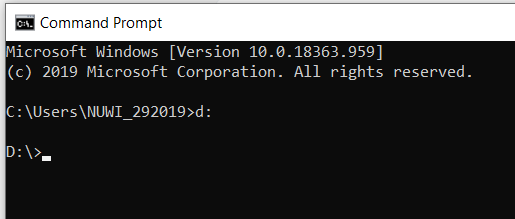
\includegraphics[width=7.15in]{images/4-2-cmdWindowPathChange} \caption{How to change the HDD drive in command prompt (if required)}\label{fig:fig4-2}
\end{figure}

\begin{enumerate}
\def\labelenumi{\alph{enumi})}
\setcounter{enumi}{2}
\tightlist
\item
  Navigate to the analysis directory using the cd (i.e.~the change
  directory) command after which you type the name of the directory. Pro
  tip: Hitting the Tab key auto-fills the folder name. Try it out, it is
  really handy!
\end{enumerate}

\begin{figure}
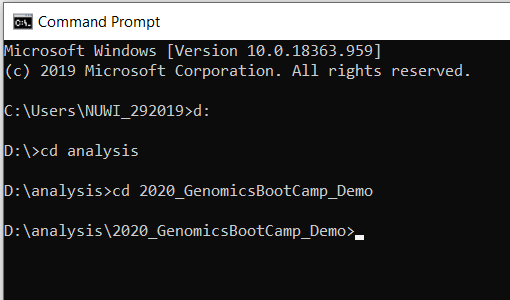
\includegraphics[width=7.08in]{images/4-3-cmdWindowPathChange2} \caption{How to navigate to the working directory}\label{fig:fig4-3}
\end{figure}

\begin{enumerate}
\def\labelenumi{\alph{enumi})}
\setcounter{enumi}{3}
\tightlist
\item
  Run the plink.exe program you copied there, as described in point 2.
  You can do this by simply typing: plink
\end{enumerate}

\begin{figure}
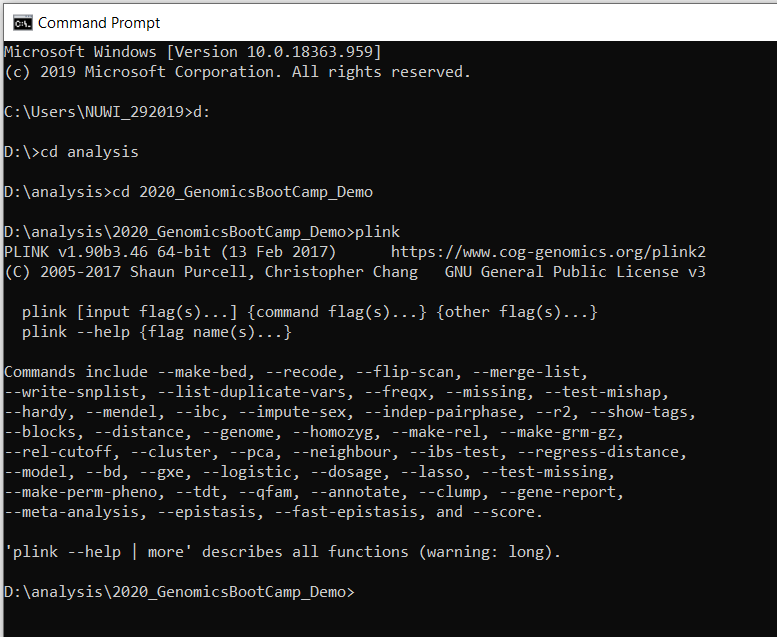
\includegraphics[width=10.79in]{images/4-4-runPlink} \caption{How to start PLINK}\label{fig:fig4-4}
\end{figure}

If your command prompt prints out the message you above you are good to
go! Congratulations!

At this point, PLINK does not do anything, because you did not include
any data. We will include some data and much more in the following
steps. Note to Linux and Mac users: You might need to run PLINK in your
terminal as ./plink Note2 to Linux (and Mac?) users: Before the first
run of the program you might need to make plink.exe executable.

\section{Exercise}\label{exercise}

It is a very useful approach to intentionally generate errors, so you
see how the program reacts. This way is you make an unintentional error,
you will see the same message as before, and you can react quicker. So
for this time:

Excercise 1) When trying to start PLINK, intentionally mistype the name,
e.g.~as pliiiink

Excercise 2) Delete the PLINK executable file from the folder and try to
run it as described in the 3d) description above

The solutions and explanations to these exercises, with a bit of bonus
content you will find on the accompanying YouTube channel.

If the embedded video does not start, click it again to ``Watch on
YouTube''. Direct link:
\url{https://www.youtube.com/watch?v=4VL4z71Ht70}

\begin{verbatim}
## PhantomJS not found. You can install it with webshot::install_phantomjs(). If it is installed, please make sure the phantomjs executable can be found via the PATH variable.
\end{verbatim}

\hypertarget{r-and-rstudio}{\chapter{R and
RStudio}\label{r-and-rstudio}}

\begin{quote}
Learning outcomes At the end of this chapter you will be able to install
R and R Studio as your integrated work environment for data processing
and visualization.
\end{quote}

Before going forward with the analysis of genomic data, I would advise
you to do one more step. You see\ldots{} Your overall goal is to make
sense of your genomic data by computing certain statistics (depending on
the goal of the study) and visualize the results. Now, PLINK can compute
many things, but surely not everything. So you probably need something
else in addition. Also, PLINK lacks any visualization capacities, so you
surely need something else for the visuals.

Here, my advice is to find an integrated work environment that could do
both computation and visualization for a wide range of analyses. Of
course, you can venture out to the World Wide Web, and/or ask your
colleagues for their recommendations. Your final choice could depend on
your previous experiences, or those of your colleagues and friends, or
even the routines at your workplace. With this choice, there is no ``one
size fits all'' solution.

My recommendation is to use the R programming language. It is easy to
use even for beginners, it is freely available, with a lot of packages
for an extremely diverse range of methodologies. In addition, it could
be used as a universal environment to run all your code (including
PLINK), so you do not need to copy-paste commands, move around files, or
other such error-prone shenanigans.

In the following part of this chapter, you will see how to install the R
work environment (four easy steps), briefly discuss how said R work
environment looks like. An example of use is demonstrated in the
\protect\hyperlink{your-first-plink-tutorial}{Your first PLINK tutorial}
chapter that shows how to run PLINK from R.

\section{Getting R and R Studio}\label{getting-r-and-r-studio}

The \emph{R programming language} comes along in a program that should
be downloaded and installed on your computer. To be very honest here,
the native form does not look so nice. It is essentially a command-line
interface that might not be friendly to beginner users (read: it is not
beginner-friendly at all). With time, you will get used to it, but if
you are at a stage figuring out what a ``working directory'' is, you
probably appreciate all the visual help and aid you can get.

The \emph{R studio} is a huge improvement in this regard. It provides
clickable insight to data, shows your script, work environment, graphs,
and help files, all on one screen. It is the work environment you use to
make your life easier.

So how to get these two beauties:

\begin{enumerate}
\def\labelenumi{\arabic{enumi})}
\item
  Go to the \href{https://www.r-project.org/}{R Project website} and
  click the Download link on top of the left pane. After choosing a
  preferred mirror site, proceed to download the R for your operating
  system, Windows, Mac, or Linux.
\item
  Install R from the downloaded file. You will be asked a bunch of
  questions during the process, but you are fine to click just ``Next''
  all the time.
\item
  Go to the \href{https://rstudio.com/products/rstudio/download/}{R
  Studio website} and download the program. You will see that there are
  paid versions as well, but the free version will be more than enough
  for you. I am using this for many years now.
\item
  Install R Studio from the downloaded file. Again, the default settings
  should be good to go.
\end{enumerate}

\section{How to use R Studio}\label{how-to-use-r-studio}

After opening R Studio, you will see a similar layout as shown in the
picture below.

\begin{figure}
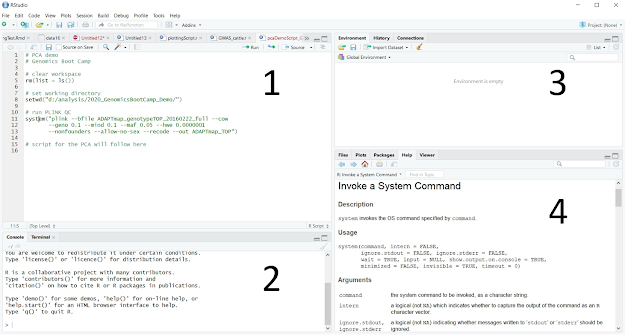
\includegraphics[width=8.68in]{images/5-1-RStudioLayout} \caption{The layout of R Studio: 1. Script editor; 2. R console; 3. Environment; 4. Help and graphs}\label{fig:fig5-1}
\end{figure}

The program itself can do a lot of things, but for now, you are fine to
know about the main parts. For your convenience, I numbered them and
will explain them briefly.

\begin{enumerate}
\def\labelenumi{\arabic{enumi})}
\item
  The part on the top left is the script editor that has an integrated
  syntax-highlighting feature. This means that comment lines, function
  names, and similar are distinguished with different colors. Moreover,
  you can run the script directly from here, so no copy-pasting is
  required. As you see, you can have multiple tabs opened at the same
  time as well. At a fresh install this part may not be visible, so just
  click File \textgreater{} New File \textgreater{} R Script to get to
  this stage.
\item
  On the bottom left is the R console itself. This is the actual R that
  you have installed previously. Here you can also see how your script
  performs, or if there are any warning or error messages to take care
  of.
\item
  On the top right there are multiple tabs. The most important one is
  the ``Environment'', which will show any data and variables you will
  work with. The data sets are also clickable, so if you want to see
  them, just click and these will be displayed in the top left part.
\item
  On the bottom right there are also multiple tabs. Two of them are of
  particular interest. The first one being the ``Help'' tab, which is
  also displayed in the picture. You see\ldots{} All R functions come
  with a help file, which you need to consult if you want to run any
  kind of analysis. The other tab of interest is ``Plots'', which will
  show you any visualizations you have created during your work.
\end{enumerate}

\section{Excercise}\label{excercise}

The exercise for this topic will be about the exploration of what R can
do. The short answer: (almost) everything. Long answer: There is a lot
of books and other resources written about it.

From the data analysis and visualization perspective, one of the options
is to use the so-called tidyverse packages. This part of R is still
relatively new and constantly developing. Still, if you are new to R, or
you have experience ``just'' with the base R, I warmly recommend
checking it out.

So what you need to do:

\begin{enumerate}
\def\labelenumi{\arabic{enumi})}
\item
  Install tidyverse. We did not go into details about package
  installation, but I firmly believe you can do it! Also, there is help
  all around.
\item
  Check out the \href{https://r4ds.had.co.nz/}{R for Data Science book},
  available for free, online. This is not about genomics, but rather on
  the use of R and tidyverse for data visualization and modification.
  There are also notes on the tidyverse installation there (chapter
  3.1.1).
\end{enumerate}

As always, you are encouraged to check out the YouTube video (below) to
compare your solutions with me and for some bonus material on the topic.

If the embedded video does not start, click it again to ``Watch on
YouTube''. Direct link:
\url{https://www.youtube.com/watch?v=nKLqqkWWyA0}

\hypertarget{genotype-files-in-practice}{\chapter{Genotype files in
practice}\label{genotype-files-in-practice}}

\begin{quote}
Learning outcomes At the end of this chapter, you will be able to
recognize and describe the format of SNP genotype files.
\end{quote}

In case you read this book from the beginning, you now have a good plan
where to place your files and the support programs installed. You only
need one more thing, and that is the data.

So where you can get some?

The good news is that due to journal and funding agency policies, and
the general goodwill of various research teams there is a lot of SNP
data available. For this introduction and also the follow-up
demonstrations we will use the
\href{http://www.goatadaptmap.org/}{AdaptMap} goat data set. This
particular data set is linked to the publication
\href{https://gsejournal.biomedcentral.com/articles/10.1186/s12711-018-0421-y}{Bertolini
et al. (2018)}

\begin{quote}
\href{https://datadryad.org/stash/dataset/doi:10.5061/dryad.v8g21pt}{DOWNLOAD
the data from here \textasciitilde{}46MB}
\end{quote}

In this post, you will see how the genomic data looks like in a PLINK
format, and how to tell its basic characteristics just by looking at it.
See!!! I told you the text editors will come in handy!

Unpack the zip file you obtained from Dryad into your working directory.
You should see something like this:

\begin{figure}
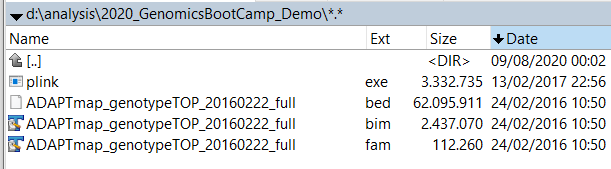
\includegraphics[width=8.49in]{images/6-1-AdaptMapGenotypeFiles} \caption{The AdaptMap goat genotype files in PLINK format}\label{fig:fig6-1}
\end{figure}

The three files contain information on animals, SNP positions, and
animals in a so-called PLINK ``binary ped'' format. This is one of the
most standard formats of the data that is efficient for computation and
storage space.

Just by looking at the file names, you can see some special
characteristics. The first one is that all three files have exactly the
same name, and differing only in the file extension. This is on purpose.
When you use the correct option in PLINK, you can refer to all three
files just by using this common name, in this case,
ADAPTmap\_genotypeTOP\_20160222\_full. This is really handy!

The second thing is maybe not so apparent, but once you have seen a few
data sets, it will become obvious. What I mean is that the file
extensions are not just some random names, but pre-defined ones from
PLINK. Also, these three belong together, and while individual files
alone could give you some information, all three are needed to analyze
the data.

A quick note here: technically it is possible to use any file name with
the right options, but why would you complicate your life (also) with
this? So I really suggest sticking to this naming convention, i.e.~the
same filename with .bim + .bed + .fam extensions.

So it is time to open the files! As all the file formats are described
on the PLINK webpage in detail, I would point out just the main things
here, and mention a few additional nuggets of information from my
experience that are not easily available elsewhere.

\section{Fam file - Info on
individuals}\label{fam-file---info-on-individuals}

We start with ADAPTmap\_genotypeTOP\_20160222\_full.fam which looks like
this:

\begin{figure}
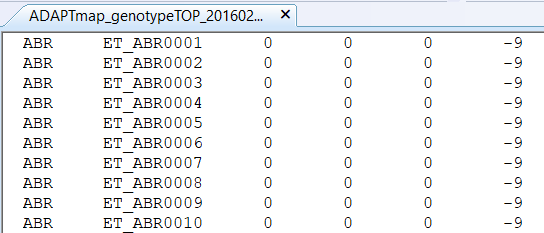
\includegraphics[width=7.56in]{images/6-2-AdaptMapFamFile} \caption{The .fam file format layout}\label{fig:fig6-2}
\end{figure}

You see that despite the funny file extension it is just a plain text
file with six columns and no header. Each column has a very specific
function that is described on the File formats webpage for .fam. What
you need to know about the respective columns is the following:

\begin{enumerate}
\def\labelenumi{\arabic{enumi})}
\item
  The first column is the family identification abbreviated as FID. As
  the PLINK software was primarily developed for genomic analyses in
  humans, which is reflected in the naming terminology and default
  settings. In the AdaptMap data set, the use of this column is to
  specify breed identity. If you look into Table 1 of the linked
  publication, you will find that the ABR abbreviation belongs to the
  Abregelle goats from Ethiopia. Using the FID column to denote breed
  information is certainly popular, but you are not limited to it. You
  can use any meaningful grouping of your data as you see fit.
\item
  The second column is the ``within family ID'', which is just simply
  called ``individual ID'' and abbreviated as IID. Although this
  phrasing might suggest that the same IID could be used with different
  FID, it is a very good idea to have unique IIDs for each individual in
  your data set. For any specification of individuals within PLINK
  however the IID always goes together with FID, so you have to devote
  sufficient attention to both anyway.
\item
  and 4) The third column is the ID of the side and the fourth column
  the ID of the dam of the animal whose IID is denoted in the second
  column. If any of the parents are genotyped their ID in the third and
  fourth columns and their IID should correspond. It is often the case
  that the parents are not known, or at the time of genotyping, there is
  not enough time to fill out the parent information and it is set to 0.
  It is not a problem in most cases, but in some types of analyses, we
  have to be aware of this and include appropriate options (e.g.~when
  looking at the minor allele frequency - don't worry about this now
  though).
\item
  Column five contains the sex information of the animal in the IID
  column. According to the built-in coding, 1 is for males, 2 for
  females, and 0 is unknown. Similar to parent information, this is also
  many times missing, usually not a problem, but specific options need
  to be included in case of any issues come up.
\item
  The sixth column is to denote the phenotype of the animal in the IID
  column. Because this is only a single column, only a single phenotype
  could be specified. In a case-control study the numerical value 1 is
  reserved for controls, and 2 for the cases. Alternatively, you can use
  any other number, including decimals for any other phenotype. In the
  case of missing values, you can use zero or minus nine. The question
  of what happens if your true phenotype measurements are 0 or -9 is
  still a mystery for me. In these cases, it is probably a good idea to
  use slightly different numbers instead.
\end{enumerate}

An additional piece of information you get from the .fam files is the
total number of individuals for which genotypes are available. This
number is corresponding to the number of lines in the .fam file. In this
case, we see that the AdaptMap data set consists of a total of 4653
genotypes!

\section{Bim file - SNP location
info}\label{bim-file---snp-location-info}

The bum file contains the locations of all SNPs in the data. When you
open it with the text editor of your choice, you will see that it is
nothing else than an ordinary text file called
ADAPTmap\_genotypeTOP\_20160222\_full.bim and looks like this:

\begin{figure}
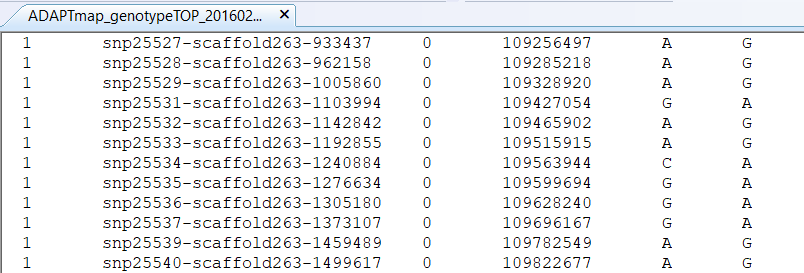
\includegraphics[width=11.17in]{images/6-3-AdaptMapBimFile} \caption{The .bim file format layout}\label{fig:fig6-3}
\end{figure}

Similar to the .fam file, the bim file has six columns, with a fixed
structure described in detail on the webpage. Some info about them in
brief:

\begin{enumerate}
\def\labelenumi{\arabic{enumi})}
\item
  The first column contains the chromosome number where the SNP is
  located. The goats have 29 so-called autosomal chromosomes and the
  number 30 is the sex chromosome. When you open a file you will see
  that it starts with a chromosome zero. These are the so-called
  unplaced SNPs, for which we know their genotype, but we are not
  entirely certain where they are on the genome.
\item
  The second column is the SNP name. This name is predefined during the
  construction of the SNP chip and fixed. If you ever want to compare
  versions of different SNP chips for the same species, the SNP overlaps
  based on their names is an excellent way to start.
\item
  The third column is the position of the SNP in Morgans or
  centimorgans, with zero value if you do not know or do not care.
  Honestly, for most of the analyses, this could be kept as zero. If you
  do some fancy stuff involving recombinations you can always amend this
  column also in existing map files.
\item
  The fourth column is the base pair coordinate of the SNP. In other
  words, you (well, not you personally, but the people who put the chip
  together) start to count from the beginning of the chromosome and for
  each SNP write down its exact location. At the beginning of each new
  chromosome, the counter resets and starts from one again. If we go
  with the example above, the SNP on the top of the list is on the
  109,256,497th position from the start of chromosome 1. Please note
  that comma or any other separators are not allowed, I use them here
  just to make the reading more convenient.
\item
  and 6) In the remaining two columns five and six are the alleles for
  respective SNPs. All SNPs on the chips are biallelic by design, so you
  always see only two alleles in each row. So this means that for each
  SNP there could be only these two characters representing the genotype
  and the character representing the missing genotypes (not shown in the
  .bim file, coded as zero by default). This is a very important concept
  that will be relevant later on when it comes to merging SNP data sets.
  Genotypes in column five usually denote the minor allele and in column
  six the major allele (more about the allele frequency in the quality
  control in chapter
  \protect\hyperlink{genotype-data-quality-control}{Genotype data
  quality control}). In some cases you also see the number 0 appearing
  e.g.~for SNP snp10412-scaffold1372-579082 right at the beginning of
  the bim file. This means that in this case, all known genotypes are
  homozygous GG, i.e.~fixed in the sample with no alternative allele.
\end{enumerate}

Similar to .fam files, you can extract one more fairly useful piece of
information just by looking at the file. Here again, the number of rows
in the .bim file shows how many SNPs are in the data set you are looking
at. For the AdaptMap data, this is 53,347 SNPs.

\section{Bed file - Individual
genotypes}\label{bed-file---individual-genotypes}

So right now you know that the files you downloaded contain genotypes
for 4653 animals, each of them genotyped for 53,347 SNPs. But you might
rightfully ask: ``Where are the genotypes for the individual animals?''

These are located in the ADAPTmap\_genotypeTOP\_20160222\_full.bed file,
but unfortunately, you can not look at them. Well\ldots{} you can, but
all you will see is something like this:

\begin{figure}
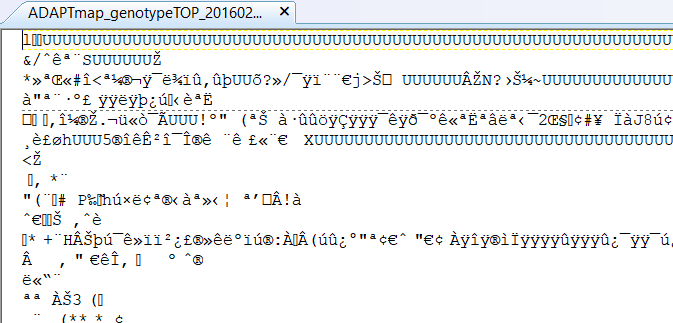
\includegraphics[width=9.35in]{images/6-4-AdaptMapBedFile} \caption{The .bed file opened with a text editor}\label{fig:fig6-4}
\end{figure}

This is because the genotypes are coded in a so-called binary format.
This not just takes a very small hard disk space, but it is processed
quicker by the computer since it's already translated from
human-readable to a machine-readable format. Of course, quite often it
is very useful to check out the individual genotypes, so to have them in
a text format is required. The non-binary file format for the genotype
is stored in the so-called ped and map files. These are also some very
well-known (I dare to say iconic) file formats and widely used in
various programs.

And how to get these files? It will be your task in your first actual
use of the PLINK program. But don't worry! I will help you.

\section{Excercise}\label{excercise-1}

Before you move on to the next section it is very useful to challenge
yourself and your understanding of the topic that was just discussed.
For this time,
\href{https://datadryad.org/stash/dataset/doi:10.5061/dryad.th092}{download
this genotype dataset from Dryad}, connected to the
\href{https://journals.plos.org/plosgenetics/article?id=10.1371/journal.pgen.1004254}{Decker
et al.(2014)} paper.

Questions to answer:

\begin{enumerate}
\def\labelenumi{\alph{enumi})}
\item
  How many animals were genotyped?
\item
  How many SNPs are available in the data set?
\end{enumerate}

After you have your answer, head over to my YouTube channel to find the
solution with some bonus content on this issue.

If the embedded video does not start, click it again to ``Watch on
YouTube''. Direct link:
\url{https://www.youtube.com/watch?v=vZyf5aXlB-k}

\hypertarget{your-first-plink-tutorial}{\chapter{Your first PLINK
tutorial}\label{your-first-plink-tutorial}}

\begin{quote}
\textbf{Learning outcomes:} At the end of this chapter, you will be able
to change genotype data formats with PLINK.
\end{quote}

In the previous posts, you read about the general suggestions for the
work environment, downloaded the PLINK software, and genotype data for a
surprisingly large number of animals. But the program was not executed
yet in any meaningful way\ldots{} But now everything will change and you
will finally run the PLINK program. Your goal will be to transform the
binary file format saved as bim, bed, and fam files to a text-based
genotype format saved as ped and map files. This exercise will also give
you a detailed description of the use of PLINK. You will see that it is
not difficult at all. Frankly, I look at the program as some kind of
building-block game. You need to know what you want to achieve and all
you need to do is add the correct elements to it. The first thing you
need to write down is some sort of base structure. In fact, you can
start with this very same line all the time and add elements to it.

But before you begin\ldots{}

\ldots{}I know, I know I am annoying with these recommendations all the
time, and you are eager to jump in\ldots{} But hear me out\ldots{} You
can type the PLINK commands directly to the command line, but don't do
that. You will see that there will be many mistakes and re-runs all the
time, and this way you will need to re-type all the time. This is a huge
loss of time. You don't want that. Open a new text file instead and
write your program script there. Ideally, this text file is saved in a
cloud storage directory, so it is being automatically backupped upon
save. Remember: the script files are very small in size, but extremely
valuable given the amount of time you invested in writing them.

\ldots{}one more piece of advice, in case you are new to scripting and
programming. You might be surprised, but the scripts you write should be
readable by the computer, but perhaps even more importantly by people,
including future you. Let me explain\ldots{} You write any script today
and you sort of know what it does. I guarantee you that if you come back
to it even after a week, you will have to spend quite some time figuring
out what it does. Not to mention if you wrote some stuff like two years
ago\ldots{} Or imagine that you have to send this script to your
colleague, who was not involved in the writing at all! If it is not
clear how to change even basic things like input file names or
locations, you are just looking for problems. So just document your code
using plain words what some crucial lines or sections do. I use the \#
hashtag sign at the beginning of each comment line to indicate it as
such. Also, lines starting with a \# are ignored in many programs, so do
not cause general errors.

Long story short: \textbf{Document your code!}

So now you will run PLINK. For real this time\ldots{} Open the command
prompt in a folder where you have the plink executable file and the
genotype data, as described before in the
\protect\hyperlink{plink---software-for-genomic-analyses}{PLINK -
Software for genomic analyses} chapter. Open a new text file and copy
the following lines in there:

\begin{Shaded}
\begin{Highlighting}[]
\CommentTok{# Change binary genotype to ped+map format}
\NormalTok{plink }\OperatorTok{--}\NormalTok{bfile ADAPTmap_genotypeTOP_20160222_full }\OperatorTok{--}\NormalTok{cow }\OperatorTok{--}\NormalTok{nonfounders }\OperatorTok{--}\NormalTok{allow}\OperatorTok{-}\NormalTok{no}\OperatorTok{-}\NormalTok{sex }\OperatorTok{--}\NormalTok{recode }\OperatorTok{--}\NormalTok{out ADAPTmap_TOP}
\end{Highlighting}
\end{Shaded}

Save the text file. From now on any change you implement will be written
to the text file first, so you can adapt easily in case of need. Copy
the whole plink line to the command prompt (without the comment line)
and press enter. You have to have 1Gb free space for the recoded file.
If everything went well, you will see this:

\begin{figure}
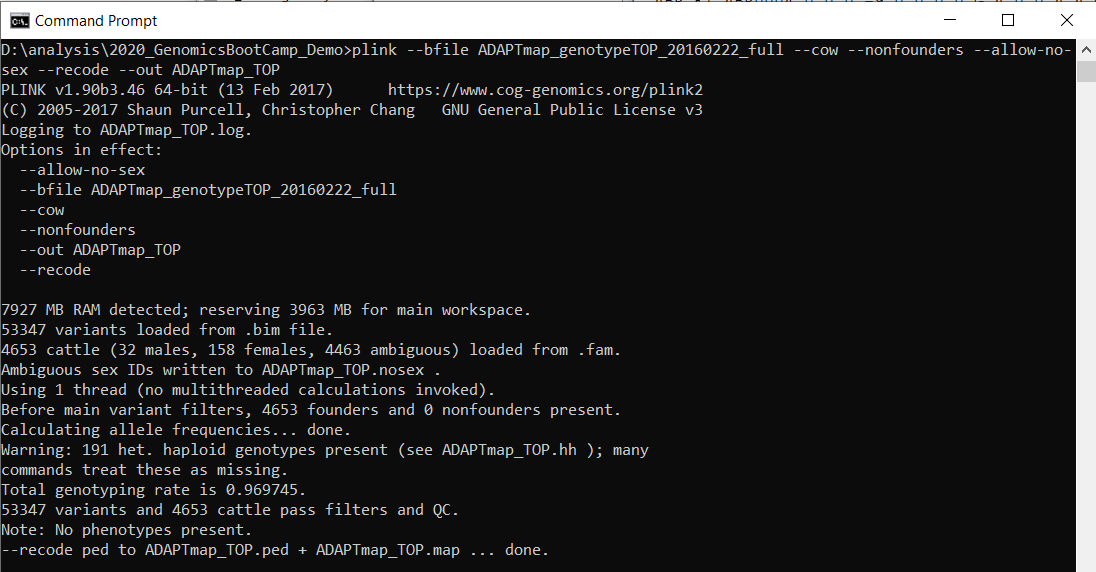
\includegraphics[width=15.22in]{images/7-1-cmdSuccessfulPlinkRun} \caption{A successful PLINK run}\label{fig:fig7-1}
\end{figure}

In the following section I will explain what you just did in two parts:

First, let's start with the PLINK options. I will list them,
simultaneously providing a link to them on the PLINK website. I will
also tell you how can you (easily?) find answers for any PLINK option.

Second, I will talk about the resulting ped and map files, including
their structure.

\section{The PLINK options}\label{the-plink-options}

I start with a general comment about the overall structure of PLINK that
you have already noticed. After the program name, there are various
options preceded by a double dash ``--''. Some
less-appropriate-text-editors like MS Word might autocorrect this to a
long dash, which will result in an error. So again, just use a proper
text editor.

The PLINK options come in two formats:

\begin{quote}
\emph{--optinName1}
\end{quote}

\begin{quote}
\emph{--optionName2 space additionalParameter(s)RelatedToOptinName2}
\end{quote}

What the options used in the previous run mean:

\href{https://www.cog-genomics.org/plink/1.9/input\#bed}{--bfile}
ADAPTmap\_genotypeTOP\_20160222\_full This is how you specify that your
input file format is a binary ped file. Because you have all three files
in the same directory as the PLINK executable, you only need to specify
the file prefix, and the program will automatically utilize everything
from the bim, bed, and fam files.

\href{https://www.cog-genomics.org/plink/1.9/input\#chr_set}{--cow} This
specifies the number of chromosomes in your data set. In case you do not
tell anything about chromosome sets, the program will use the human
genome as a default setting. Now you might have noticed that we deal
with goats, but we specify --cow here. This time we played on the fact
that bot cattle and goats have 60 chromosomes. In case you use another
organism, you either specify that option, or a new setting using
--chr-set

\href{https://www.cog-genomics.org/plink/1.9/filter\#nonfounders}{--nonfounders}
Do you remember when I talked about parental information in the fam
file? This option is related to bypass any animals with missing parent
information being treated as founders. Now, when you read the
description on the website, you will also see that it is considered only
in a few cases anyway. The thing is, however, that I tend to forget to
use the handle in specific cases, and then spend \emph{a lot} of time
figuring out what went wrong. This is the pesky type of error when there
is no error message, but the outcome is just incorrect. So to avoid all
of this, I use --nonfounders in all my plink lines.

\href{https://www.cog-genomics.org/plink/1.9/filter\#allow_no_sex}{--allow-no-sex}
Similar to parental info, the info on sex is also many times missing. As
it might or might not be problematic for certain analyses, I have
decided to include this option in all my PLINK lines. The justification
is the same as for --nonfounders.

\href{https://www.cog-genomics.org/plink/1.9/data\#recode}{--recode}
This very simple command is the one that actually does all the work. By
putting this in your code you specify that you want to have \emph{ped}
and \emph{map} files as output.

\href{https://www.cog-genomics.org/plink/1.9/general_usage\#out}{--out}
ADAPTmap\_TOP Specifies the file name for newly created files.

So now you might have a very valid question: ``This is all nice, but how
do I find descriptions for other types of analyses I want to do?''

The two possibilities are:

\begin{enumerate}
\def\labelenumi{\arabic{enumi})}
\tightlist
\item
  If you know exactly what are you looking for, you can use the handy
  search tool at the bottom of the left panel on the website, as shown
  in the picture. The result(s) below the search box are clickable links
  to the resource.
\end{enumerate}

\begin{figure}
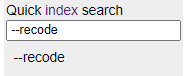
\includegraphics[width=2.61in]{images/7-2-plinkHelpSearch} \caption{Find this bottom left on the PLINK website to get help}\label{fig:fig7-2}
\end{figure}

\begin{enumerate}
\def\labelenumi{\arabic{enumi})}
\setcounter{enumi}{1}
\tightlist
\item
  If you don't know what you are looking for, try to explore the topics
  discussed on the left panel on the PLINK website, check other people's
  code, or simply ask colleagues how to do something. Alternatively, you
  can also try to fish for answers in
  \href{https://www.cog-genomics.org/plink/1.9/index}{the list of all
  PLINK options}, using Ctrl+F text search capacities of your browser.
  You can also get there by clicking the ``index'' keyword link above
  the search bar.
\end{enumerate}

Here I would note that PLINK can do \emph{many} things, but certainly
not \emph{everything}. So do not expect to be a one-stop-shop for all of
your genomic analysis needs. It is just a tool. A handy one, but still
just one out of many.

\section{The ped and map file format}\label{the-ped-and-map-file-format}

In this section, we will take a brief look at the newly created files
and tell something about their structure.

You might have noticed that there are a few new files created in the
same directory you have run the program. From these files, the ones with
file extension .ped and .map are the most important.

The \href{https://www.cog-genomics.org/plink/1.9/formats\#map}{.map}
file is very similar to the previously described .bim file, just without
the last two columns with genotypes.

The \href{https://www.cog-genomics.org/plink/1.9/formats\#ped}{.ped}
file structure is essentially the concatenation of the .fam file (one
line per individual), followed by human-readable genotypes in text
format. Every two columns represent one SNP in a space-delimited format.

To open the .map file should be no problem. The .ped file however is
nearly 1Gb in size! I got the ``File too big to be opened'' error
message with Notepad++, but the TextPad opened it without problems
(after a bit of waiting time, might be machine-dependent, you will see a
small progress bar bottom left).

\section{How to run PLINK from R}\label{how-to-run-plink-from-r}

As a practical demonstration of work with genomic data in R Studio, we
will use PLINK example we discussed before in this chapter. With this,
you will see the elements that need to be included to integrate the
PLINK script to R and also prepare you for the grand finale of the first
section - the PCA analysis.

The script we will be running is the following:

\begin{Shaded}
\begin{Highlighting}[]
\CommentTok{# clear workspace}
\KeywordTok{rm}\NormalTok{(}\DataTypeTok{list =} \KeywordTok{ls}\NormalTok{())}

\CommentTok{# set working directory}
\KeywordTok{setwd}\NormalTok{(}\StringTok{"d:/analysis/2020_GenomicsBootCamp_Demo/"}\NormalTok{)}

\CommentTok{# run PLINK QC}
\KeywordTok{system}\NormalTok{(}\StringTok{"plink --bfile ADAPTmap_genotypeTOP_20160222_full --cow --nonfounders             --allow-no-sex --recode --out ADAPTmap_TOP"}\NormalTok{)}
\end{Highlighting}
\end{Shaded}

From my personal experience in learning and teaching genomic data
analysis to people of wide-ranging levels of experience, just telling
you to copy-paste-and-run-the-script does not lead anywhere. So I will
explain the most important elements of this script.

All lines starting with a hashtag \# are comment lines. As I explained
in a previous post, these are essential in all scripts. You need to be
very clear what each part of the script is doing, which is much easier
if you comment on it. The line rm(list = ls()) is a very useful one that
I use in all my R scripts. It deletes everything from the workspace.
This way I know that there are no pesky leftovers from previous analyses
that might compromise my runs. (Ever had an experience of ``The script
was running before and it is not running now!''? This might be because
of unintended data sets in the work environment.)

The setwd() is an R function that (as the name implies) sets the working
directory for this session. The working directory is the place, where R
will look for all the data for the analyses and place any output files
if you do not specify otherwise. By default, this is a directory
somewhere on your system drive. While it will work, I strongly suggest
changing it to comply with your own file organization structure in a
custom directory, as discussed before. You will need to change this for
your run. Just put the PATH to your working directory containing PLINK
and the genotype files between the quotation marks. Please note that R
uses the opposite slashes as Windows.

You probably recognize the contents of the system() function. This is
the exact copy of the PLINK command we used before, again between
quotation marks. That's right! It is this easy to run PLINK from R. With
the use of this function, the R opens the system command line, runs the
line of code, and closes the command line.

Each line of the script above could be run separately. To do this, just
put your cursor to the line you want to execute, and press the ``Run''
button in the top right corner. Alternatively, you can use the even
better and arguably quicker method of simultaneously pressing Ctrl+Enter
(Command+Enter in Mac).

\section{Exercise}\label{exercise-1}

Phewww\ldots{} You made it to the end of this unexpectedly long
description! Congratulations! But to really drive home the message and
lock the knowledge in your memory, I have a small task for you.

You see, the PLINK file formats are really popular, but there are many
others out there. The good news is, that you can use PLINK to transform
files to other popular formats. One of them is undoubtedly the so-called
variant call format that is the standard output file from whole-genome
sequencing pipelines, and a possible input to some other programs. So
your task is to change the ADAPTmap file to vcf file format.

\emph{Hint:} if I were you, I would explore the various options of the
\href{https://www.cog-genomics.org/plink/1.9/data\#recode}{--recode}
option on the website. \emph{wink-wink}

As always, you can compare your solution to the one on YouTube. The
video also contains some bonus information on related problems you might
face during analyses, so make sure to check it out regardless.

If the embedded video does not start, click it again to ``Watch on
YouTube''. Direct link:
\url{https://www.youtube.com/watch?v=c1LSFiv9CxY}

\hypertarget{genotype-data-quality-control}{\chapter{Genotype data
quality control}\label{genotype-data-quality-control}}

\begin{quote}
\textbf{Learning outcomes:} At the end of this chapter you will be able
to filter out low-quality genotypes from your data using PLINK.
\end{quote}

At this point, you already know how the genomic data looks like
(\protect\hyperlink{genotype-files-in-practice}{Genotype files in
practice} chapter) and how to process it with PLINK
(\protect\hyperlink{your-first-plink-tutorial}{Your first PLINK
tutorial} chapter). So it is reasonable to assume that you want to do
some kind of real analysis at some point. But here I am to tell you: Do
not rush it!

Before you do any kind of analysis, you need to check the quality of
your genotype data and delete the sketchy parts. The good old saying
``Garbage in, garbage out.'' is valid also here, so you want to avoid
this by doing quality control (QC). This chapter will tell you how, why,
and when to do certain moves.

We will start with a toy example and then move to the implementation in
PLINK.

\section{A toy example}\label{a-toy-example}

In this example, we will consider a data set with five individuals each
of them genotyped for five SNPs. The genotypes themselves are in
numerical coding, 11 and 22 being the two homozygous, 12 the
heterozygous, and 00 coded as missing.

\begin{figure}
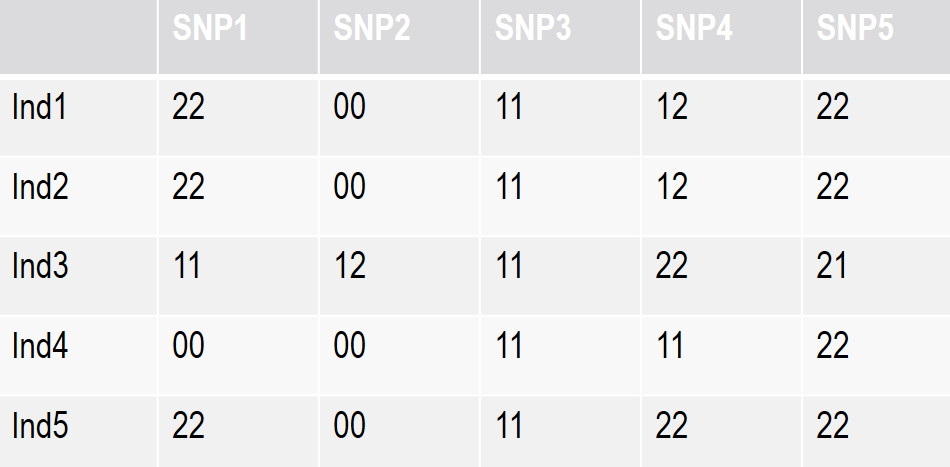
\includegraphics[width=13.19in]{images/8-1-qualityControlToyExample} \caption{A small scale example for genotype quality control}\label{fig:fig8-1}
\end{figure}

\subsection{Missingness per SNP}\label{missingness-per-snp}

Overall, the SNP genotyping platform is very reliable and delivers
stable results when it comes to determining genotypes. Of course, it is
not flawless. One of the most frequent problems is that some of the SNPs
are just not well genotyped in the entire population. These should be
removed to improve the overall data quality.

Of course, we can not remove every SNP that has any missing value, as
this way we would purge the entirety of our data. As a comproimse, we
define thresholds instead. The funny thing about these thresholds is
that no rule would firmly set which ones to use. So you are free to
define them as long as you remain within ``reasonable'' bounds. To find
out what ``reasonable'' means, it is perhaps a good idea to study the
literature for your species of interest.

In this toy example, we will go with a 20\% threshold. In other words,
we would delete any SNP with more than 20\% missing SNPs. In our case,
SNP2 would be deleted.

\subsection{Missingness per
individual}\label{missingness-per-individual}

The reliability of SNP chips is also high when it comes to individual
genotypes. In some cases, however, some of the individuals contain a
large number of missing SNPs. The reason could be low DNA sample
quality, wrong chip type used (e.g.~cattle chip for deer samples), or
other technical issues. Regardless of the reason, you should delete the
worst offenders from your data set, not to compromise the overall
quality of your results.

In our toy example, we go with a 30\% threshold, which means that
individual 4 is deleted.

An interesting question is the follow-up of the quality control steps.
If we would define a more conventional 10\% threshold in our toy
example, this would remove all genotypes. If we implement the filtering
first by SNP (removing the problematic SNP2), and the filtering for
individuals just after that, we are in much better shape.

\subsection{Minor allele frequency}\label{minor-allele-frequency}

You can compute the proportion of any allele in any SNP based on the set
of genotype data you have. For example in SNP4 we have five genotypes
with a total of 10 alleles, four of them are Allele1 (40\% or 0.4), and
six of them Allele2 (60\% or 0.6).

The Allele occurring less frequently will be the so-called minor allele,
and the proportion of its occurrence called minor allele frequency
(MAF). In the case of SNP4, the Allele1 is the minor allele, with a
frequency of 0.4.

Limitations on the minor allele frequencies are done similarly as
previously. You just define a number and every SNP with MAF below this
number gets deleted. If you want to get rid only of the fixed SNPs, you
specify a MAF threshold of 0.

\subsection{Adherence to Hardy-Weinberg
distribution}\label{adherence-to-hardy-weinberg-distribution}

The quality control based on Hardy-Weinberg (H-W) distribution is a bit
trickier to explain. You might know the definition of
\href{https://www.khanacademy.org/science/biology/her/heredity-and-genetics/a/hardy-weinberg-mechanisms-of-evolution}{the
Hardy-Weinberg rule} from population genetics which states that genetic
variation (thus allele and genotype frequencies) in a population will
remain constant unless certain disturbing elements are introduced. This
also means that when we know the allele frequencies for p and q, the
genotype frequencies will be defined as p\textsuperscript{2}, 2pq, and
q\textsuperscript{2}.

\textbf{A more detailed example on Hardy-Weinberg limitation}

Let's say the frequency of allele A (p in the equation)is 0.4, and that
of allele B (q in the equation) is 0.6. This means for the H-W scenario
the genotype frequencies will be 0.16 for AA, 0.48 for AB, and 0.36 for
BB. This also means that in a population of e.g.~1000 individuals with
the mentioned allele frequencies we expect to see 160 AA, 480 AB, and
360 BB individuals. Of course, we rarely see exact H-W distributions in
real populations. The question then becomes, what is the extent of the
difference between the expected H-W proportions in each SNP, and the
observed proportions in the reality?

The way to provide a threshold to exclude unwanted SNPs is via a p-value
threshold. If the expected and observed genotype frequencies are
``equal'' based on an equilibrium exact test with the significance
(p-value) you provide, the SNP is kept during the quality control. If
there are large differences between the expected and observed
frequencies, the SNP is deleted.

From personal experience, I know that referring to p-values as ``high''
or ``low'' could be confusing, as you can never be too certain if this
is meant as the numerical value or the strictness level (with lower
p-values are being more strict). So to be very straightforward: you
delete much more SNPs (i.e.~you do a stricter QC) with the H-W
significance threshold of e.g.~0.001 than if you set this to
e.g.~0.000000001.

\section{How QC works in PLINK}\label{how-qc-works-in-plink}

The implementation of the quality control steps in PLINK is easy.
Remember the line in \protect\hyperlink{your-first-plink-tutorial}{Your
first PLINK tutorial}? All you need to do is to include the
corresponding PLINK options to that line with the quality control
parameters of your choice. You could of course search for them on the
options list I showed you, but for now, I am going to give you a head
start:

Missingness per SNP:
\href{https://www.cog-genomics.org/plink/1.9/filter\#missing}{--geno}
\emph{value}

Missingness per individual:
\href{https://www.cog-genomics.org/plink/1.9/filter\#missing}{--mind}
\emph{value}

Minor allele frequency:
\href{https://www.cog-genomics.org/plink/1.9/filter\#maf}{--maf}
\emph{value}

Hardy-Weinberg threshold:
\href{https://www.cog-genomics.org/plink/1.9/filter\#hwe}{--hwe}
\emph{value}

An additional very frequently used option is
\href{https://www.cog-genomics.org/plink/1.9/filter\#autosome}{--autosome}.
By including this option you automatically keep only SNPs on the
autosomal chromosomes. So any unplaced SNPs or those on the sex
chromosomes get removed.

\textbf{Caution!} The --maf option is not considered in founder animals,
i.e.~those with unknown parents. Please note that the parentage
information is many times skipped from data sets out of convenience or
because it is not available. To include such animals in the quality
control, use the
\href{https://www.cog-genomics.org/plink/1.9/filter\#nonfounders}{--nonfounders}
option in your script.

\section{Exceptions from SNP quality
control}\label{exceptions-from-snp-quality-control}

When \emph{NOT} to include certain parameters into the QC?

Depending on the analysis you want to perform, you might not want to
include some of the parameters mentioned above. This is because by doing
so, you might be deleting the very results you are looking for.

Let me explain\ldots{}

For example, you want to do anything with runs of homozygosity (ROH) -
to look for long homozygous segments, that could be also fixed in the
population. Implementing any kind of MAF filtering would get rid of
fixed or highly homozygous SNPs. In the next step of your analysis, you
would then proceed to look for fixed or highly homozygous regions on the
genome\ldots{} Ehm\ldots{} You see how this went wrong, right?

Another example is if you are interested to look for previously unmapped
disorders via the approach called ``missing homozygosity''. This method
is based on the fact that you see much less homozygous genotypes for a
certain allele compared to the expectations. The reason for the apparent
lack of homozygotes might be because these alleles are in fact
deleterious recessives. So any individual having them in homozygous form
dies before it gets a chance to be genotyped. Of course, this also means
that there will be an imbalance between observed and expected genotypes.
The very result you are looking for! In case you apply the
Hardy-Weinberg filtering however, you delete these from your records in
the quality control step, as they are out of HWE expectations\ldots{}

So I hope you get the picture\ldots{} Quality control is necessary, but
a cautious implementation is advised.

\section{Exercise}\label{exercise-2}

You made it to the end! Congratulations!

You might have noticed that I did not give a full PLINK line on how to
implement the QC to your existing script. That is because I want YOU to
do it! That's right! This way you will reinforce your knowledge on QC
and get a bit more practice with the implementation.

Take the PLINK line from your first PLINK tutorial with the ADAPmap
data, and extend it with the following QC parameters:

Missingness per SNP: 0.1; Missingness per individual: 0.1; Minor allele
frequency: 0.05

The questions are: What was the number of animals and SNPs before and
after quality control? How many individuals and SNPs were removed due to
the different criteria? Optional: See what happens if you include also a
Hardy-Weinberg threshold: 0.0000001

As always, you can compare your solution with mine. In the video link
below I discuss this exercise.

If the embedded video does not start, click it again to ``Watch on
YouTube''. Direct link:
\url{https://www.youtube.com/watch?v=QR80Y0Xhrg4}

\chapter{Principal component analysis
(PCA)}\label{principal-component-analysis-pca}

\begin{quote}
\textbf{Learning outcomes:} At the end of this chapter, you will be able
to perform and visualize the results from a principal component analysis
(PCA).
\end{quote}

In this chapter, we will do a principal component analysis (PCA) based
on quality-controlled genotype data. From the technical side, we
willcontinue to work in R.

\section{Run a PCA in R}\label{run-a-pca-in-r}

The PCA itself is a way to visualize complex systems in a simple way. In
our case, we want to show relationships between the worldwide goat
populations genotyped in the ADAPTmap project. After the quality
control, we have 4532 animals left. If we compute genetic distances
(with PLINK), we get a matrix of 4532 by 4532 animals, with more than 10
million pairwise combinations. So a ``rather'' long list to scroll
through, let alone make sense of it.

Fortunately, we can apply some clever statistical methods to simplify it
for us. We will lose some precision and nuances about the relationships
between breeds, but in exchange, we can see everything in one figure.

\subsection{PCA in R - The script}\label{pca-in-r---the-script}

For completeness, I show the complete R code.

\begin{Shaded}
\begin{Highlighting}[]
\CommentTok{# PCA demo}
\CommentTok{# Clear workspace}
\KeywordTok{rm}\NormalTok{(}\DataTypeTok{list =} \KeywordTok{ls}\NormalTok{())}
\CommentTok{# Set working directory}
\KeywordTok{setwd}\NormalTok{(}\StringTok{"d:/analysis/2020_GenomicsBootCamp_Demo/"}\NormalTok{)}
\CommentTok{# Run PLINK QC}
\KeywordTok{system}\NormalTok{(}\StringTok{"plink --bfile ADAPTmap_genotypeTOP_20160222_full --cow --autosome --geno 0.1 --mind 0.1 --maf 0.05 --nonfounders --allow-no-sex --recode --out ADAPTmap_TOP"}\NormalTok{)}

\NormalTok{######################################}
\CommentTok{# Principal Component Analysis - PCA #}
\NormalTok{######################################}

\NormalTok{## Genetic distances between individuals}
\KeywordTok{system}\NormalTok{(}\StringTok{"plink --cow --allow-no-sex --nonfounders --file ADAPTmap_TOP --distance-matrix --out dataForPCA"}\NormalTok{)}

\NormalTok{## Load data}
\NormalTok{dist_populations<-}\KeywordTok{read.table}\NormalTok{(}\StringTok{"dataForPCA.mdist"}\NormalTok{,}\DataTypeTok{header=}\NormalTok{F)}
\NormalTok{### Extract breed names}
\NormalTok{fam <-}\StringTok{ }\KeywordTok{data.frame}\NormalTok{(}\DataTypeTok{famids=}\KeywordTok{read.table}\NormalTok{(}\StringTok{"dataForPCA.mdist.id"}\NormalTok{)[,}\DecValTok{1}\NormalTok{])}
\NormalTok{### Extract individual names }
\NormalTok{famInd <-}\StringTok{ }\KeywordTok{data.frame}\NormalTok{(}\DataTypeTok{IID=}\KeywordTok{read.table}\NormalTok{(}\StringTok{"dataForPCA.mdist.id"}\NormalTok{)[,}\DecValTok{2}\NormalTok{])}
  
\NormalTok{## Perform PCA using the cmdscale function }
\CommentTok{# Time intensive step - takes a few minutes with the 4.5K animals}
\NormalTok{mds_populations <-}\StringTok{ }\KeywordTok{cmdscale}\NormalTok{(dist_populations,}\DataTypeTok{eig=}\NormalTok{T,}\DecValTok{5}\NormalTok{)}

\NormalTok{## Extract the eigen vectors}
\NormalTok{eigenvec_populations <-}\StringTok{ }\KeywordTok{cbind}\NormalTok{(fam,famInd,mds_populations}\OperatorTok{$}\NormalTok{points)}

\NormalTok{## Proportion of variation captured by each eigen vector}
\NormalTok{eigen_percent <-}\StringTok{ }\KeywordTok{round}\NormalTok{(((mds_populations}\OperatorTok{$}\NormalTok{eig)}\OperatorTok{/}\KeywordTok{sum}\NormalTok{(mds_populations}\OperatorTok{$}\NormalTok{eig))}\OperatorTok{*}\DecValTok{100}\NormalTok{,}\DecValTok{2}\NormalTok{)}
\end{Highlighting}
\end{Shaded}

\subsection{PCA in R - The
explanation}\label{pca-in-r---the-explanation}

As you see there are several steps required to get all the data that
could be later visualized.

The computation of genetic distances is done by PLINK, via the
\href{https://www.cog-genomics.org/plink/1.9/distance\#ibs_matrix}{--distance-matrix}
option. It creates the already mentioned huge matrix of numbers, saved
in a text file \emph{dataForPCA.mdist}. Go ahead and open it with the
text editor of your choice to check it out! Quite a lot of numbers,
right?

We will simplify it using multidimensional scaling in R. To do this, we
will first load the text file to R, along with the names of breeds
(\emph{fam} variable) and individual IDs (\emph{famInd} variable).

The next step will be the heavy lifting, the multidimensional scaling,
and the computation of eigenvectors. This is done using the
\emph{cmdscale()} function, taking into account the first five principal
components. As a follow up we merge the PCA results with the breed and
individual ID information (\emph{eigenvec\_populations}) and compute the
variance explained by each principal component (\emph{eigen\_percent}).
This last bit of information on the percent of variance explained is not
strictly necessary for the visualization, but it will be a nice addition
to our plot.

\section{Visualize PCA results}\label{visualize-pca-results}

At this point, we have a lot of numbers and results, but still, no
picture to show to our boss, supervisors, extended family in annual
gatherings, and other conventional or unconventional places where we
want to show off with our results. It is time to change it now!

\subsection{PCA visualization - The
script}\label{pca-visualization---the-script}

\begin{Shaded}
\begin{Highlighting}[]
\CommentTok{# Visualize PCA in tidyverse}
\CommentTok{# Load tidyverse}
\ControlFlowTok{if}\NormalTok{ (}\OperatorTok{!}\KeywordTok{require}\NormalTok{(}\StringTok{"tidyverse"}\NormalTok{)) \{}
  \KeywordTok{install.packages}\NormalTok{(}\StringTok{"tidyverse"}\NormalTok{, }\DataTypeTok{dependencies =} \OtherTok{TRUE}\NormalTok{)}
  \KeywordTok{library}\NormalTok{(tidyverse)}
\NormalTok{\}}

\CommentTok{# PCA plot}
\KeywordTok{ggplot}\NormalTok{(}\DataTypeTok{data =}\NormalTok{ eigenvec_populations) }\OperatorTok{+}
\StringTok{ }\KeywordTok{geom_point}\NormalTok{(}\DataTypeTok{mapping =} \KeywordTok{aes}\NormalTok{(}\DataTypeTok{x =} \StringTok{`}\DataTypeTok{1}\StringTok{`}\NormalTok{, }\DataTypeTok{y =} \StringTok{`}\DataTypeTok{2}\StringTok{`}\NormalTok{,}\DataTypeTok{color =}\NormalTok{ famids), }\DataTypeTok{show.legend =} \OtherTok{FALSE}\NormalTok{ ) }\OperatorTok{+}\StringTok{ }
\StringTok{ }\KeywordTok{geom_hline}\NormalTok{(}\DataTypeTok{yintercept =} \DecValTok{0}\NormalTok{, }\DataTypeTok{linetype=}\StringTok{"dotted"}\NormalTok{) }\OperatorTok{+}\StringTok{ }
\StringTok{ }\KeywordTok{geom_vline}\NormalTok{(}\DataTypeTok{xintercept =} \DecValTok{0}\NormalTok{, }\DataTypeTok{linetype=}\StringTok{"dotted"}\NormalTok{) }\OperatorTok{+}
\StringTok{ }\KeywordTok{labs}\NormalTok{(}\DataTypeTok{title =} \StringTok{"PCA of wordwide goat populations"}\NormalTok{,}
    \DataTypeTok{x =} \KeywordTok{paste0}\NormalTok{(}\StringTok{"Principal component 1 ("}\NormalTok{,eigen_percent[}\DecValTok{1}\NormalTok{],}\StringTok{" %)"}\NormalTok{),}
    \DataTypeTok{y =} \KeywordTok{paste0}\NormalTok{(}\StringTok{"Principal component 2 ("}\NormalTok{,eigen_percent[}\DecValTok{2}\NormalTok{],}\StringTok{" %)"}\NormalTok{)) }\OperatorTok{+}\StringTok{ }
\StringTok{ }\KeywordTok{theme_minimal}\NormalTok{()}
\end{Highlighting}
\end{Shaded}

\subsection{PCA visualization - The
explanation}\label{pca-visualization---the-explanation}

The ggplot2 package from the tidyverse will be used for visualization.
If you have done the exercise at the end of the
\protect\hyperlink{r-and-rstudio}{R and RStudio} chapter you already
have it installed, so you just need to load. If not, you can do it now.

The first part of the script is a very neat way of making sure
everything is in place. I use this in all my R scripts. In short, it
checks if the package is already installed on your computer. If yes, it
proceeds to load it, in not installs it (if it is on CRAN), and then
proceeds to load. You can easily adapt it for any other R package by
changing the package name.

The next bit of code is the visualization itself, in a mixture of base R
and tidy coding styles. We will plot the first and second principal
components from the \emph{eigenvec\_populations} file. Here I would
underline that naming columns as numbers is not ideal, and should be
avoided in general. To keep this script as simple as possible, we will
go with these rather unfortunate names generated by the
\emph{cmdscale()} function.

Each breed will have a different color, to better visualize the groups.
We will switch off the legend on the figure. If it is on, the legend
would completely overtake the screen, given a large number of breeds.
But if you feel adventurous, go ahead and change it to \emph{show.legend
= TRUE}.

With \emph{geom\_hline()} and \emph{geom\_vline()} we add a horizontal
and vertical line at 0 for each axis to make the plot nicer. With
\emph{labs()} we add the figure title, and the axis names including the
percentages of variance explained. The \emph{theme\_minimal()} is purely
an aesthetical tuning of the figure. Again, just go ahead and
\href{https://ggplot2.tidyverse.org/reference/ggtheme.html}{change it to
some other one}, if you want.

\subsection{PCA visualization - Comparison to published
results}\label{pca-visualization---comparison-to-published-results}

If everything went well, you see the following plot in R

\begin{figure}
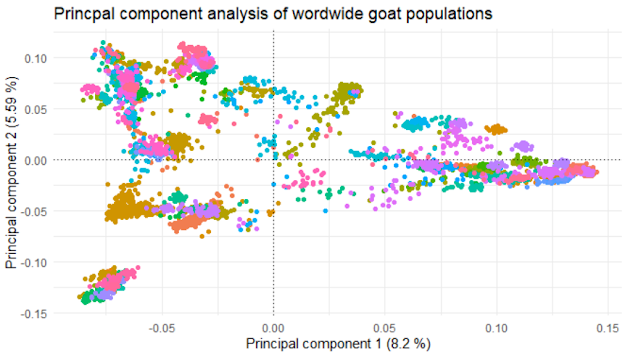
\includegraphics[width=8.68in]{images/9-1-resultsPcaGoats} \caption{Results of the PCA analysis}\label{fig:fig9-1}
\end{figure}

Nice, isn't it? Personally, I like it a lot!

During these sessions, we have produced a similar graph to the
researchers working on the data initially. I will put it below and make
some comparisons between the two.

\begin{figure}
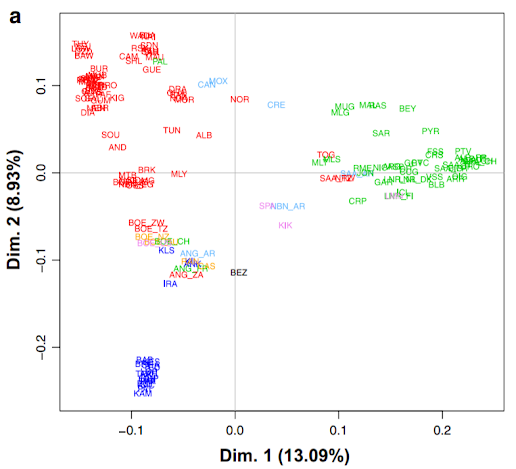
\includegraphics[width=7.17in]{images/9-2-resultsPcaPaper} \caption{Results of the PCA analysis from Colli et al. (2018)}\label{fig:fig9-2}
\end{figure}

The figure above is from
\href{https://gsejournal.biomedcentral.com/track/pdf/10.1186/s12711-018-0422-x}{Colli
et al. (2018), published in Genetics, Selection, Evolution} (open
access), figure 4a.

You see that the general shape of the two graphs is virtually identical,
which is kind of expected, as we used the same initial data and same
methods. There are a few minor differences though, worth pointing out.

Maybe the most striking one is the difference in explained variance
shown on the axes. This might be due to the differences in quality
control. If you check out the Methods section of Colli et al. (2018),
you will see that they looked at the data from a variety of different
angles, not just missingness. Also, this is a good example of what other
factors could be taken into account in QC, so it is worthwhile to check
it out anyway.

The other issue is that in the paper there are much fewer data points.
This is because only the middle point, i.e.~one point for each breed is
visualized. Additionally, they have avoided the necessity of the legend
by putting the breed abbreviations straight in the figure. Still, many
of them are overlapping and unreadable, but arguably better than a
legend with hundreds of entries.

The third thing I want to point out is the color scheme. In our case,
there is a different color for each breed. This leads to virtually
indistinguishable colors for some of the breeds. The problem is even
more serious for people with any form of color blindness. Yes, it is
pretty but otherwise utterly unusable. In Colli et al. (2018) they use
color codes for the continents, adding yet another nice piece of
information to the figure: red=Africa, green=Europe, blue=West Asia,
pink=North America, light blue=South America, orange=Oceania, black=wild
goats.

\section{\texorpdfstring{\sout{Exercise}
Summary}{Exercise Summary}}\label{exercise-summary}

If you have followed along with the other posts, you know that I usually
give you a small exercise at the end. It will not be so in this case.
Yes, I could come up with another freely available data set and ask you
to do a PCA for it.

But in this case, I will not do that.

This chapter is the final piece in a workflow, where I wanted to
describe how to process SNP genomic data, without any previous
experience. Well\ldots{} With knowledge of the theory side, but no
experience in practical data handling and analysis.

Yes, many other things need to be said and done to increase your
proficiency. But considering that you started with no previous practical
experience, we have to also acknowledge that you have come a long way.

Well done! Congratulations on your achievement!

At this point my Excercise for you, if you really want to have one, is
to \emph{celebrate}. Maybe not by throwing a big party, but in a small
personal way. Treat yourself with a chocolate or something, take some
time off, play a game, think about the work-life balance.

If you liked these chapters,
\href{https://www.youtube.com/channel/UCXuX-kQ1TbKHWeB75NgmhlA}{consider
subscribing to my YouTube channel} and
\href{https://twitter.com/GaborM_ABG}{follow me on Twitter}. These are
just two simple clicks for you, but for me are an indication of interest
and motivation to go forward!

This is of course not the end! I plan to follow up and extend the book
and also on the
\href{https://www.youtube.com/channel/UCXuX-kQ1TbKHWeB75NgmhlA}{YouTube
channel} with various topics related to genetics and genomics. So stay
tuned!

As for now, thank you for your time, and have a nice day!

If the embedded video does not start, click it again to ``Watch on
YouTube''. Direct link:
\url{https://www.youtube.com/watch?v=l5afbHnw6Uw}

\bibliography{book.bib,packages.bib}

\end{document}
